% TU Delft Beamer template
% Author: Maarten Abbink
% Delft University of Technology
% March 2014
% Version 2.0
% Based on original version 1.0 of Carl Schneider
\documentclass{beamer}
\usepackage[english]{babel}
\usepackage{graphicx}
\usepackage{algorithm,algorithmic}
%\usepackage[compatibility=false]{caption}
%\usepackage{subcaption}
\setbeamertemplate{caption}{\raggedright\insertcaption\par}
\setlength{\abovecaptionskip}{0pt} 
\usepackage{calc}
\usepackage[absolute,overlay]{textpos}
\mode<presentation>{\usetheme{tud}}
\usepackage[T1]{fontenc}
%\usetheme{Torino}
\usepackage{arev}
%\usepackage{mathtools}
%\newcommand{\defeq}{\vcentcolon=}
%\newcommand{\eqdef}{=\vcentcolon}
%\title[MSc Colloquium]{Reinforcement Learning for Tracking Control in Robotics}
\title[MSc Colloquium]{\fontsize{10}{4}\selectfont Reinforcement Learning for Tracking Control in Robotics}

%\subtitle
\institute[TU Delft]{\fontsize{8}{4}\selectfont Delft University of Technology}

\author[Yudha Prawira Pane]{\fontsize{8}{4}\selectfont Yudha Prawira Pane \hspace{3.05cm} Supervisors: Prof. Dr. Robert Babu\v{s}ka}
%\author{\fontsize{8}{4}\selectfont Yudha Prawira Pane}
%\author{\begin{tabular}{cc} 
%		Author:      & Me \\ [1ex] 
%		Supervisors: & First\\
%		& Second
%	\end{tabular}}
\date[\today]{\fontsize{8}{4}\selectfont \today \hspace{5.15cm} Subramanya P. Nageshrao}
%\author{Prof. Dr. Robert Babu\v{s}ka}
% Insert frame before each subsection (requires 2 latex runs)
\AtBeginSubsection[] {
	\begin{frame}<beamer>\frametitle{\titleSubsec}
		\tableofcontents[currentsection,currentsubsection]  % Generation of the Table of Contents
	\end{frame}
}
% Define the title of each inserted pre-subsection frame
\newcommand*\titleSubsec{Next Subsection}
% Define the title of the "Table of Contents" frame
\newcommand*\titleTOC{Outline}

% define a symbol which can be removed if you don't need it
\newcommand{\field}[1]{\mathbb{#1}}
\newcommand{\Zset}{\field{Z}}

\begin{document}
	
	{
		% remove the next line if you don't want a background image
		\usebackgroundtemplate{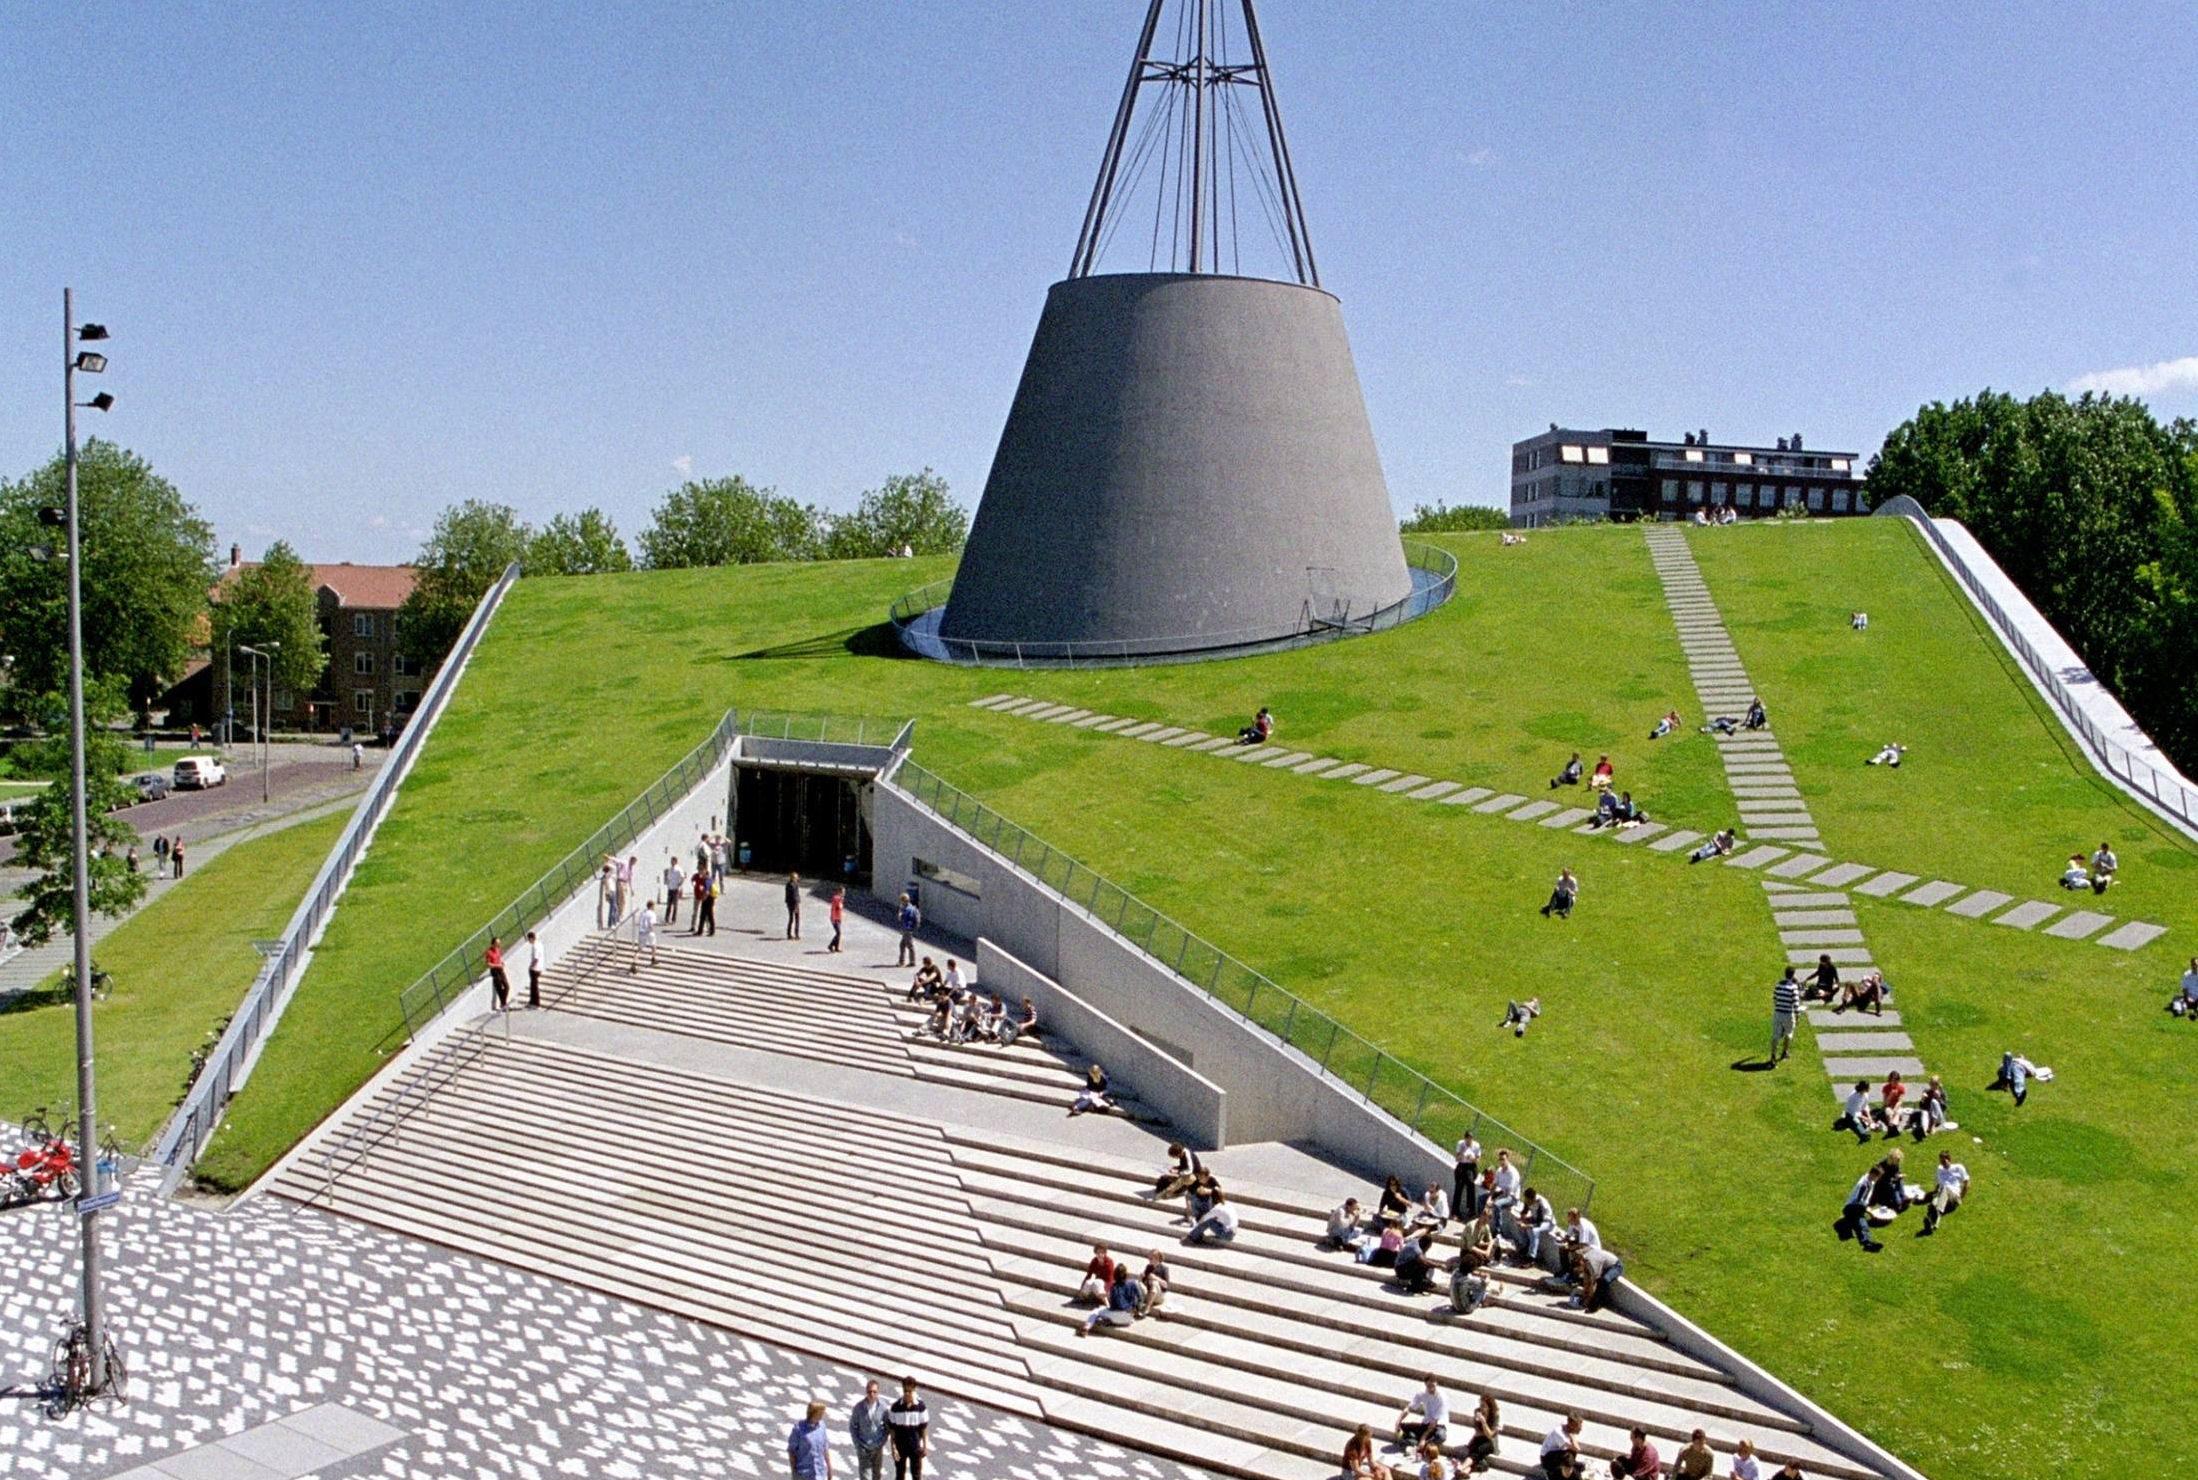
\includegraphics[width=\paperwidth,height=\paperheight]{images/background-titlepage.jpg}}%
		\setbeamertemplate{footline}{\usebeamertemplate*{minimal footline}}
		\frame{\titlepage}
	}
	
	{\setbeamertemplate{footline}{\usebeamertemplate*{minimal footline}}
		\begin{frame}\frametitle{\titleTOC}
			\tableofcontents
		\end{frame}
	}
	
	\section{Basic of Reinforcement Learning (RL) \& Tracking Control}
	\begin{frame}\frametitle{Motivation of RL}
		\begin{itemize}
			\item Inspired by how living animals learn
			\pause
			\item Learning through interaction with environment
			\pause
			\begin{figure}
				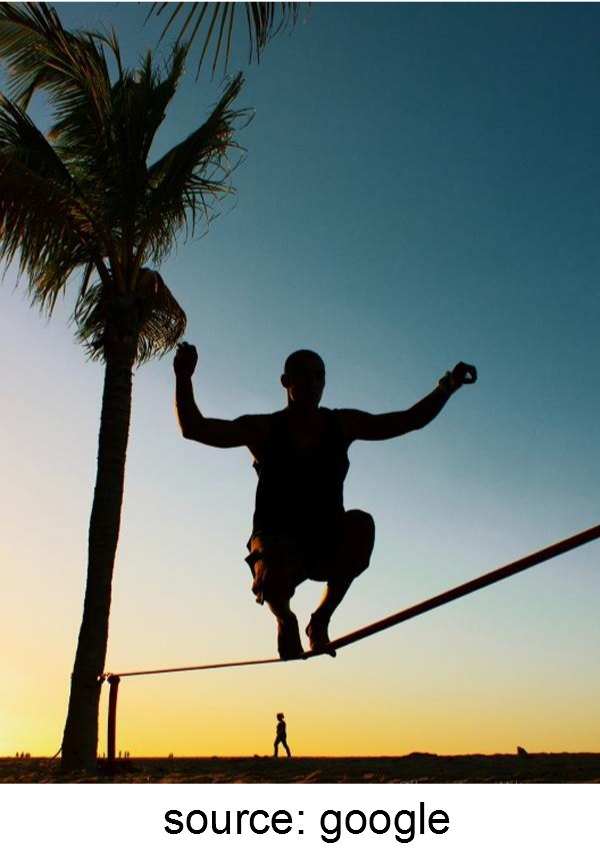
\includegraphics[width=0.30\linewidth]{images/slacklining} \hspace{5mm}
				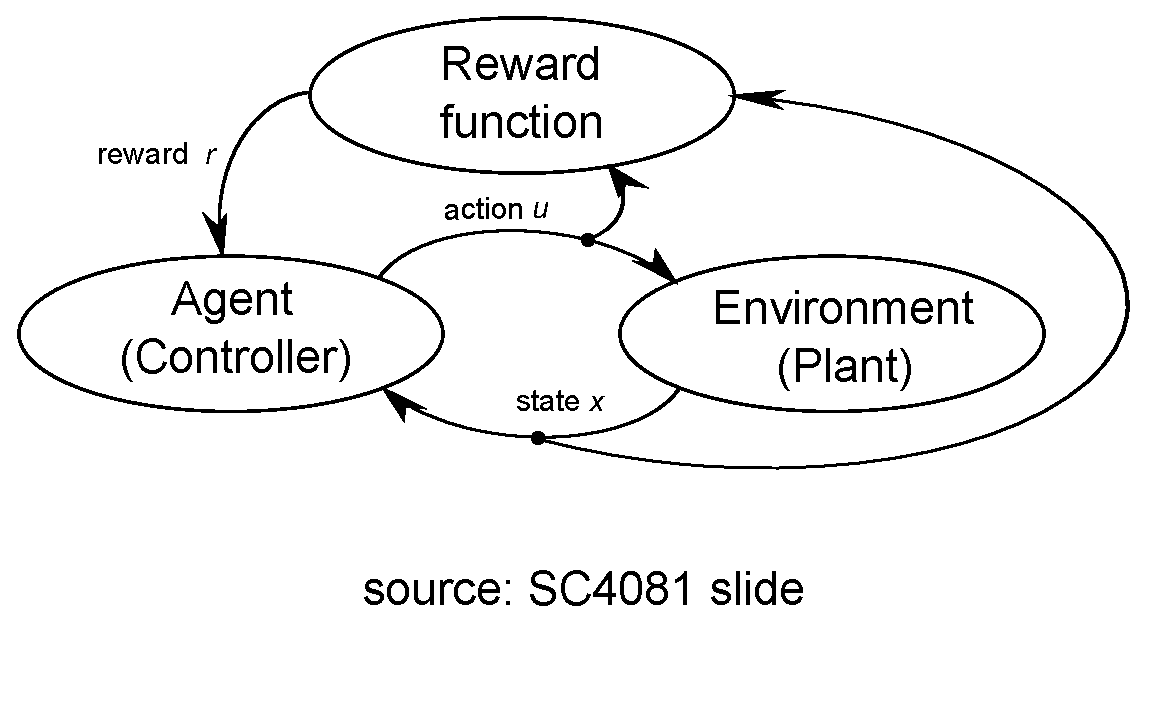
\includegraphics[width=0.60\linewidth]{images/rl_diagram}
			\end{figure}
			\pause
			\item Introduce the reward / reinforcement signal
		\end{itemize}
	\end{frame}
	
	
	\begin{frame}\frametitle{Mathematical Formalization of RL}
		\begin{definition}
			\fontsize{9}{4}\selectfont 
			A Markov Decision Process (MDP) is defined as a tuple $ \left\langle X, U, \bar{f}, \rho\right\rangle  $ where
			\begin{itemize}
				\item $ X $ = state space
				\item $ U $ = action space
				\item $ \bar{f} : X \times U \rightarrow  X $ = system dynamics
				\item $ \rho: X \times U \rightarrow \mathbb{R} $ = reward (cost) function
			\end{itemize}
		\end{definition}
		\pause
		\begin{definition}
			\fontsize{9}{4}\selectfont
			System and policy dynamics are defined as:
			\begin{equation}
			x_{k+1} = \bar{f}(x_k,u_k) = f(x_k) + g(x_k)u_k 			
			\end{equation}
			\begin{equation}
			u_{k+1} = \pi(x_k,u_k) 	
			\end{equation}
			\begin{equation}
			r_{k+1} = \rho(x_k,u_k)	
			\end{equation}		
		\end{definition}
	\end{frame}
	
	\begin{frame}\frametitle{Mathematical Formalization of RL (2)}
		\begin{definition}
			\fontsize{9}{4}\selectfont
			Formulize goal as return $ R $
			\begin{equation}
			R_k = r_k + r_{k+1} + r_{k+1} + \dots + r_T 
			\end{equation}
			Discounted return:		
			\begin{equation}
			R_k = r_{k+1} + \gamma r_{k+2} + \gamma^2r_{k+3} + \dots = \sum_{j=0}^{\infty}\gamma^jr_{k+j+1}
			\end{equation}		
		\end{definition}
		\pause
		\begin{definition}
			\fontsize{9}{4}\selectfont
			Value function $ V $ measures how a good is it to be at a certain state x 
			\begin{equation}
			V(x_{k}) = \rho(x_k,u_k) + \gamma \rho(x_{k+1},u_{k+1}) + \gamma^2 \rho(x_{k+2},u_{k+2}) + \dots 			
			\end{equation}
			\begin{equation}
			V(x_{k}) = \rho(x_k,u_k) + \gamma V(x_{k+1}) 			
			\end{equation}
		\end{definition}
	\end{frame}
	
	\begin{frame}\frametitle{Mathematical Formalization of RL (3)}
		How to obtain an optimal policy $ \pi^* $? \\
		First, an exact value function $ V$ $ \forall x \in \mathcal{X} $ must be found
		\begin{definition}
			Bellman optimality principle:
			\begin{equation}
			V^*(x_{k}) = \underset{u_k}{\text{min}} \hspace{1mm} \Big[ \rho(x_k,u_k) + \gamma V^*(x_{k+1}) \Big] 			
			\end{equation}
			\begin{equation}
			\pi^*(x_{k-1}) = u^*_k = \text{arg} \underset{u_k}{\text{min}} \hspace{1mm} \Big[ \rho(x_k,u_k) + \gamma V^*(x_{k+1}) \Big] 				
			\end{equation}		
		\end{definition}
	\end{frame}
	
	\begin{frame}\frametitle{Solutions to RL problem}
		\vspace{2mm}
		\fontsize{8}{4}\selectfont 
	 	Dynamic Programming (DP):
	 	\begin{itemize}
	 		\item needs system model
%	 		\item can be implemented in offline and online fashion
	 		\item example: policy iteration (PI)
	 	\end{itemize}
		\pause
		\begin{algorithm}[H]
			\begin{algorithmic}[1]    			
				\fontsize{8}{4}\selectfont 
				\STATE \textbf{Initialization:} 
				\STATE \hspace{2mm} Start from an admissible policy $ \pi$, assign $ V^{\pi}(x) \leftarrow 0$  
				\REPEAT    			
				\STATE \textbf{Policy Evaluation:} 
				\REPEAT 	    			    
				\STATE 	$ \Delta $ $ \leftarrow $ 0 
				\STATE 	\textbf{For each} $ x \in \mathcal{X} $ :
				\STATE 	\hspace{5mm} $ v $ $ \leftarrow $ $ V^{\pi}(x) $ 
				\STATE 	\hspace{5mm} $ V^{\pi}(x) \leftarrow \rho(x, \pi(x)) +\gamma V^{\pi}(x') $ 
				\STATE 	\hspace{5mm} $ \Delta = $ max$ (\Delta, |v-V^{\pi}(x)|) $
				\UNTIL {$ \Delta  <  \varepsilon $ (a small positive number)}
				
				\STATE \textbf{Policy Improvement:} 
				\STATE \textbf{For each} $ x \in \mathcal{X} $ : 
				\STATE \hspace{5mm} $ \pi(x)=$  arg $\underset{u}{\text{min}} \hspace{1mm} \rho(x, u) +\gamma V^{\pi}(x') $  
				\UNTIL{$ \pi $ converges}
			\end{algorithmic}
			\caption{Policy Iteration}
		\end{algorithm}
	\end{frame}
							
	\begin{frame}\frametitle{Solutions to RL problem (2)}
		\vspace{3mm}
		\fontsize{8}{4}\selectfont 
		Temporal Difference (TD)
		\begin{itemize}
			\item does not need system model
			%	 		\item can be implemented in offline and online fashion
			\item examples: Q-learning, actor-critic 
		\end{itemize}	
		\only<-1>{	
				\begin{figure}
					\includegraphics<1>[width=0.6\linewidth]{images/actorCritic} 			
					\caption{\fontsize{8}{4}\selectfont Actor-critic structure (source: SC4081 slide)}
				\end{figure}
			}
	\end{frame}
			
	\begin{frame}\frametitle{Solutions to RL problem (3)}
		\vspace{3mm}
		\fontsize{8}{4}\selectfont
		Actor critic method
		\begin{itemize}		 	
			\item suitable for continous state and action space e.g. robotics
			\item parameterize actor and critic using function approximators
		\end{itemize}
		\begin{algorithm}[H]
			\begin{algorithmic}[1]    			
				\fontsize{8}{4}\selectfont 
				\STATE \textbf{For every trial:}
				\STATE  Initialize $x_0$ and $u_0 = \tilde{u}_0$
				\REPEAT
				\STATE apply $u_k$, measure $x_{k+1}$, receive $r_{k+1}$ 
				\STATE choose next action $ u_{k+1} = \hat{\pi}(x_{k+1}, \psi_k) + \tilde{u}_{k+1} $ 
				\STATE $ \delta_k = r_{k+1} + \hat{V}(x_{k+1}, \theta_k) \hat{V}(x_{k}, \theta_k) $ 
				\STATE $ \theta_{k+1} = \theta_k + \alpha_c\delta_k \frac{\partial \hat{V}(x,\theta)}{\partial \theta} \bigg|_{x=x_k, \theta \theta_k}$ 
				\STATE $ \psi_{k+1} = \psi_k + \alpha_c\delta_k \frac{\partial \hat{V}(x,\psi)}{\partial \psi} \bigg|_{x=x_k, \psi = \psi_k}$
				\UNTIL{terminal state}				
			\end{algorithmic}
			\caption{Actor-critic algorithm}
		\end{algorithm}
	\end{frame}	
				
	\begin{frame}\frametitle{Tracking Control}
		Typical tracking controllers:
		\begin{itemize}
			\item Open-loop control 
			\item State/Output Feedback control (e.g. PID controller)
			\item Feedback + feedforward control (e.g. LQT optimal controller)
		\end{itemize}
		\vspace{3mm}
		\textbf{Drawback:} even the best of the 3 only performs as good as the model!
	\end{frame}
	
	\begin{frame}\frametitle{Research Question}
		The following research question is raised: \\
		\vspace{5mm}
		\hspace{5mm} \textit{"Is it possible to improve the tracking performance of a nominal controller using Reinforcement Learning?"}
	\end{frame}
			%\subsection{Section 1 - Subsection 2}
			
	\section{Experimental Setup: 3D Printing Robot System}
	\begin{frame}\frametitle{3D Printing Robot}
		\vspace{2mm}
		\fontsize{9}{4}\selectfont 
		\begin{itemize}
			\item The UR5 robot with unknown internal controller
			\item 4 types of command:
			\begin{itemize} \fontsize{8}{4}\selectfont  
				\item Tool Position $ (x, y, z) $ in meter \vspace{0.5mm}
				\item Tool Velocity $ (\dot{x}, \dot{y}, \dot{z}) $ in meter/s \vspace{0.5mm}
				\item Joint Position $ (q_1, q_2, q_3 , q_4, q_5, q_6)$ in rad \vspace{0.5mm}
				\item Joint velocity $ (\dot{q_1}, \dot{q_2}, \dot{q_3} , \dot{q_4}, \dot{q_5}, \dot{q_6})$ in rad/s
			\end{itemize} \vspace{1mm}
			\item The laser scanner \vspace{1mm}
			\item The 3D Print head					
		\end{itemize}
		\pause
		\begin{figure}
		\centering
		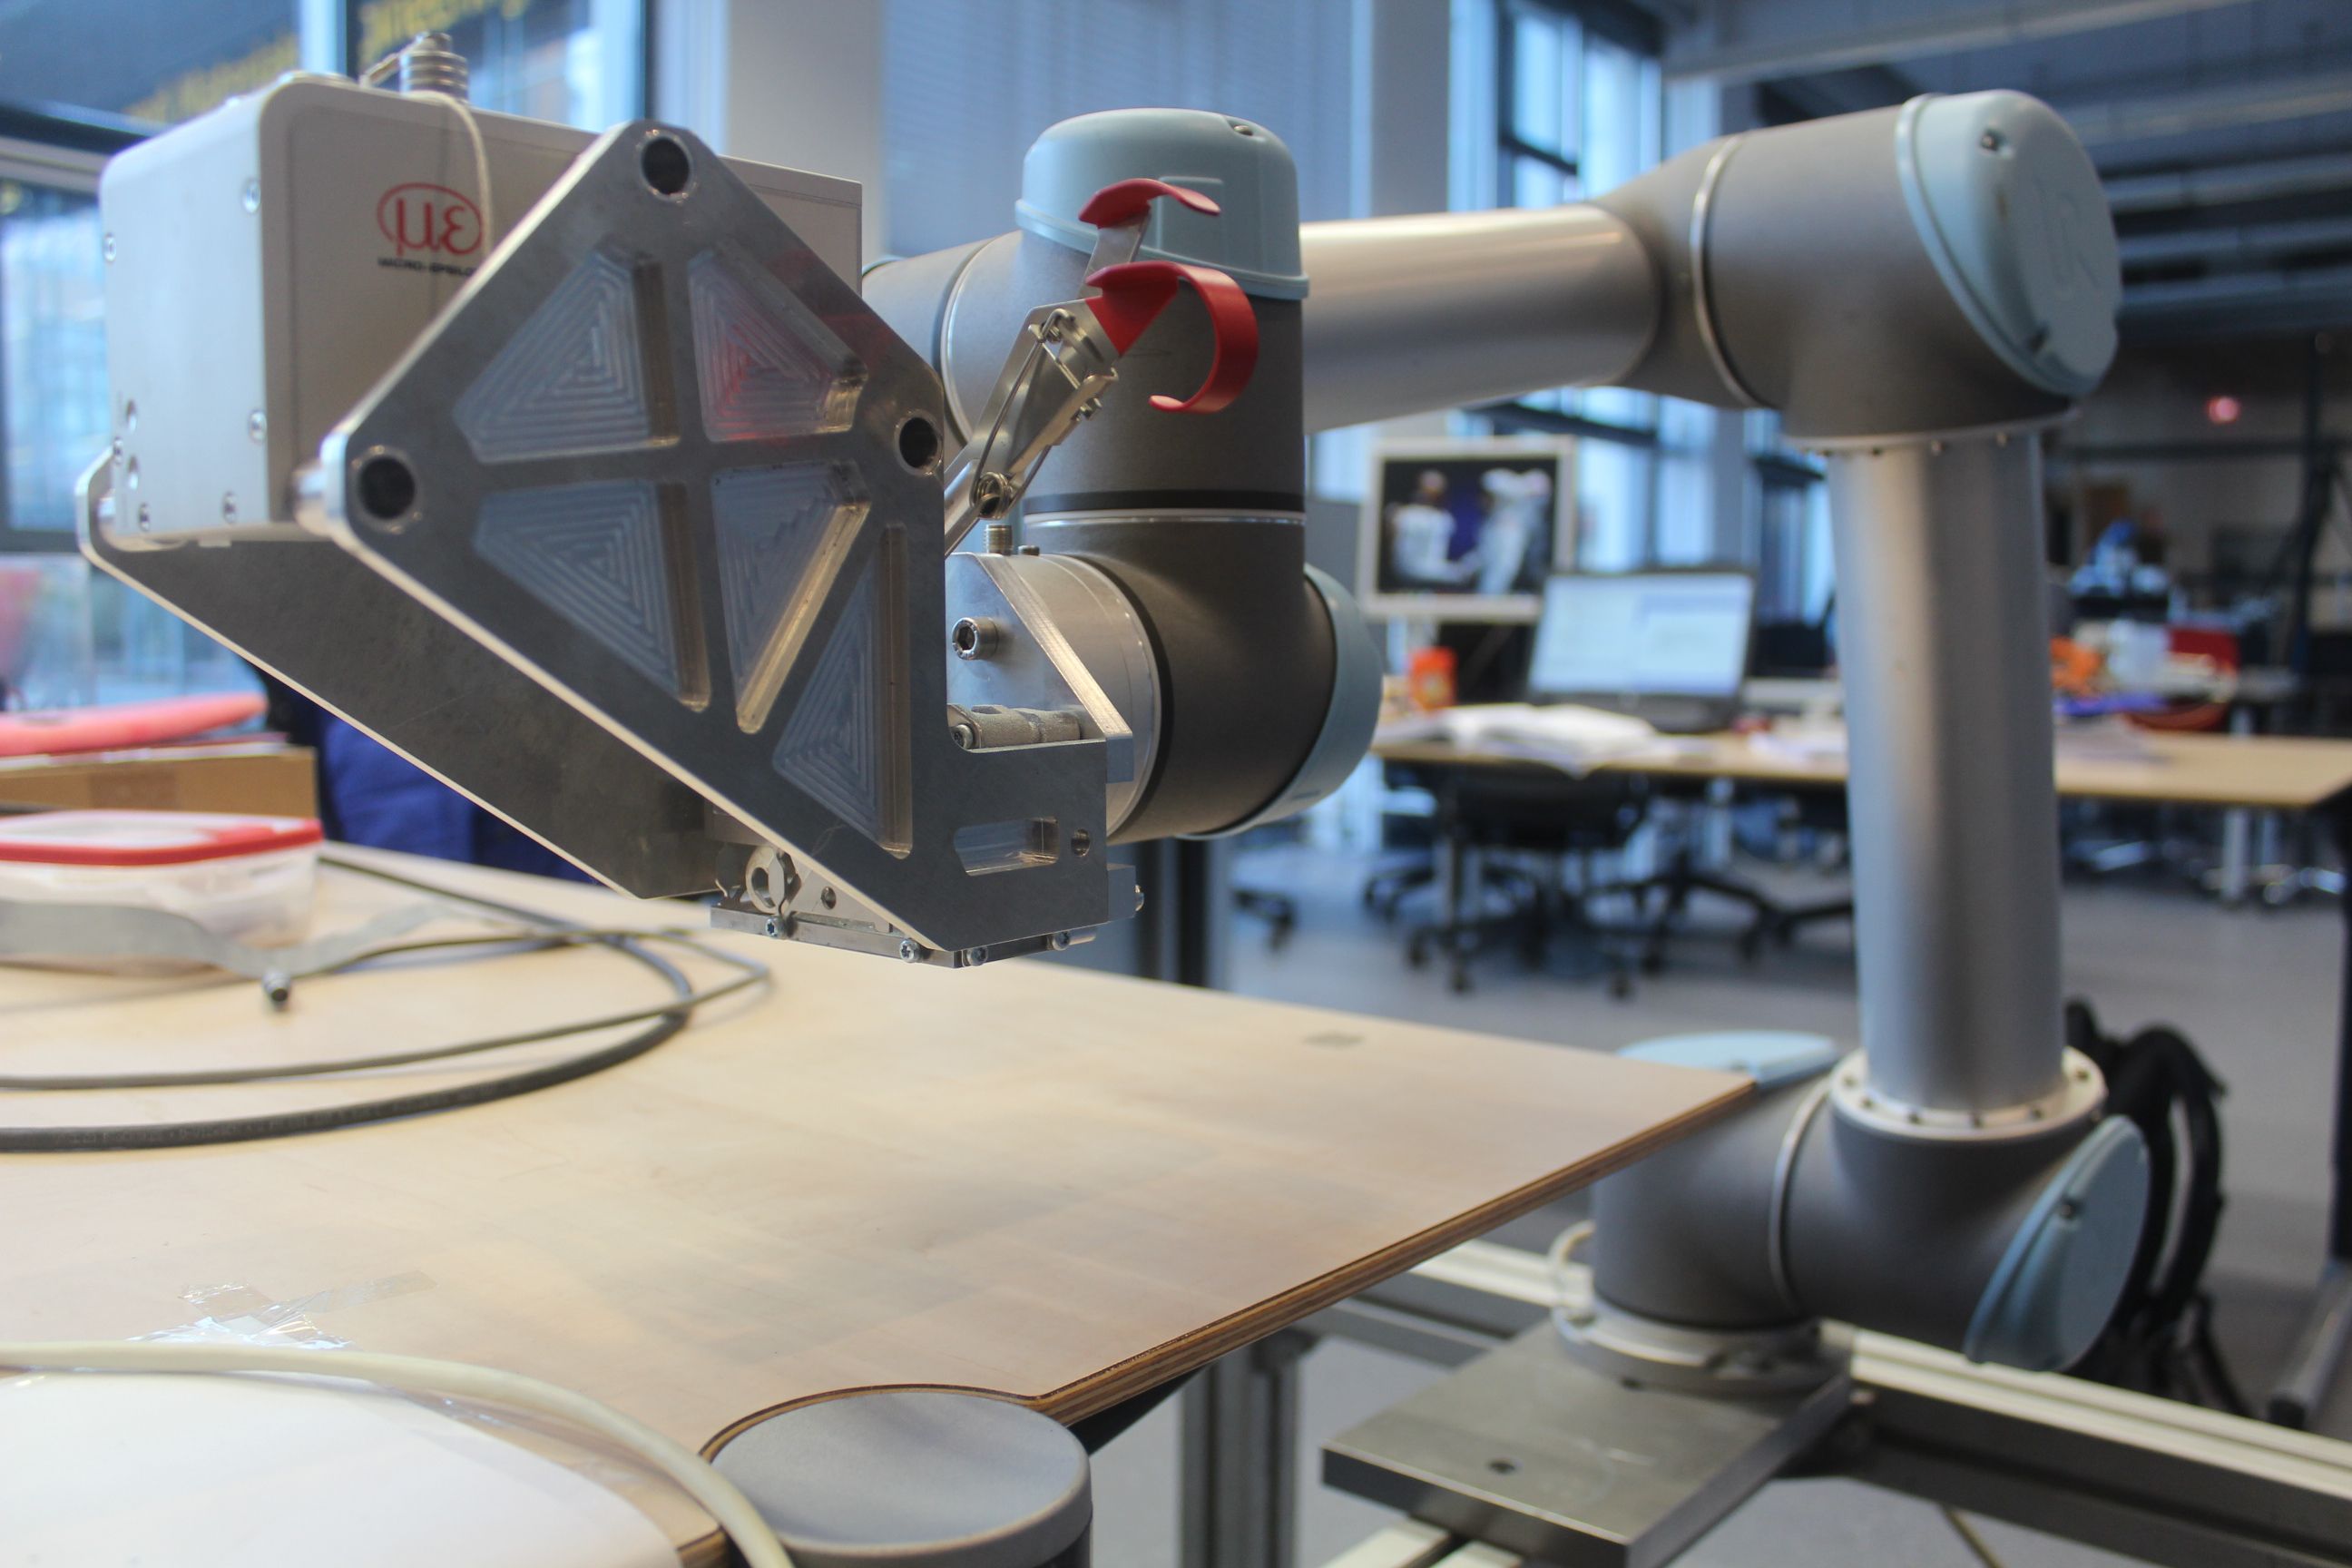
\includegraphics[width=0.53\linewidth]{images/IMG_9011}
		\caption{}
		\label{fig:IMG_9011}
		\end{figure}
	\end{frame}

	\begin{frame}\frametitle{3D Printing Robot: system identification}
		\begin{itemize}
			\item Subspace identification
				\begin{center}
					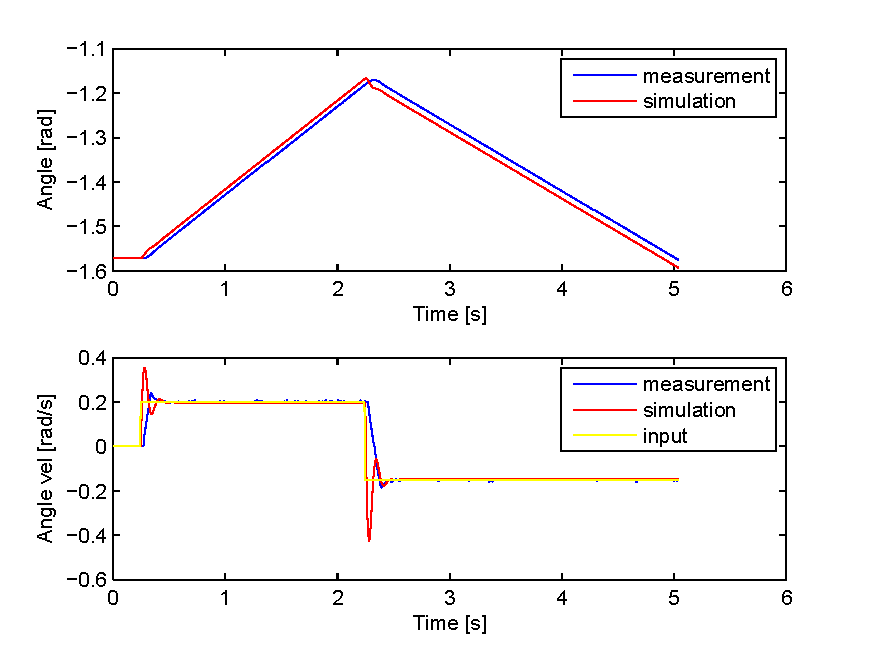
\includegraphics[width=0.53\linewidth]{images/Joint1}
				\end{center}

	\end{itemize}
			\begin{table}
				\fontsize{7}{4}\selectfont 
				\caption{\fontsize{8}{4}\selectfont  \textbf{Table 1.} VAF scores of the simulated outputs for all joints}	
				\centering
				\begin{tabular}{|c|c|c|}
					\hline Joint & Position  & Velocity \\ 
					\hline 1 & 98.64 & 87.33 \\ 
					\hline 2 & 98.05 & 88.33 \\ 
					\hline 3 & 98.55 & 88.47 \\ 
					\hline 4 & 98.97 & 89.50 \\ 
					\hline 5 & 99.46 & 90.32 \\ 
					\hline 6 & 98.87 & 85.13 \\ 
					\hline 
				\end{tabular} 
				\label{tab:vaf}
			\end{table}
							
	\end{frame}
			
			\begin{frame}\frametitle{3D Printing Robot: MPC controller}
				\vspace{2mm}
				\begin{itemize}
					\fontsize{8}{4}\selectfont
					\item test a simple straight trajectory along X-axis
					\item compares MPC with previously mentioned controllers
					
%					\begin{table}[h]
%						\centering
%						\caption{The difference between maximum and minimum values of Y-axis trajectory with different control methods}
%						\begin{tabular}{|c|c|c|}
%							\hline
%							Control method & speed & jitter's amplitude (mm) \\
%							\hline		
%							& $ \times $1 & 0.635678\\
%							Tool Position & $ \times $2 & 0.670974\\
%							& $ \times $4 & 0.624456\\
%							\hline		
%							& $ \times $1 & 0.529104\\
%							Tool Velocity & $ \times $2 & 0.376090\\
%							& $ \times $4 & 0.320906\\
%							\hline		
%							& $ \times $1 & 0.550691\\
%							Joint Velocity & $ \times $2 & 0.522474\\
%							& $ \times $4 & 0.490630\\				
%							\hline
%							\ac {MPC} & $ \times $1 & 0.120889 \\
%							\hline
%							
%						\end{tabular}
%						\label{tab:y_jitter}
%					\end{table}
					\begin{figure}
						\centering
						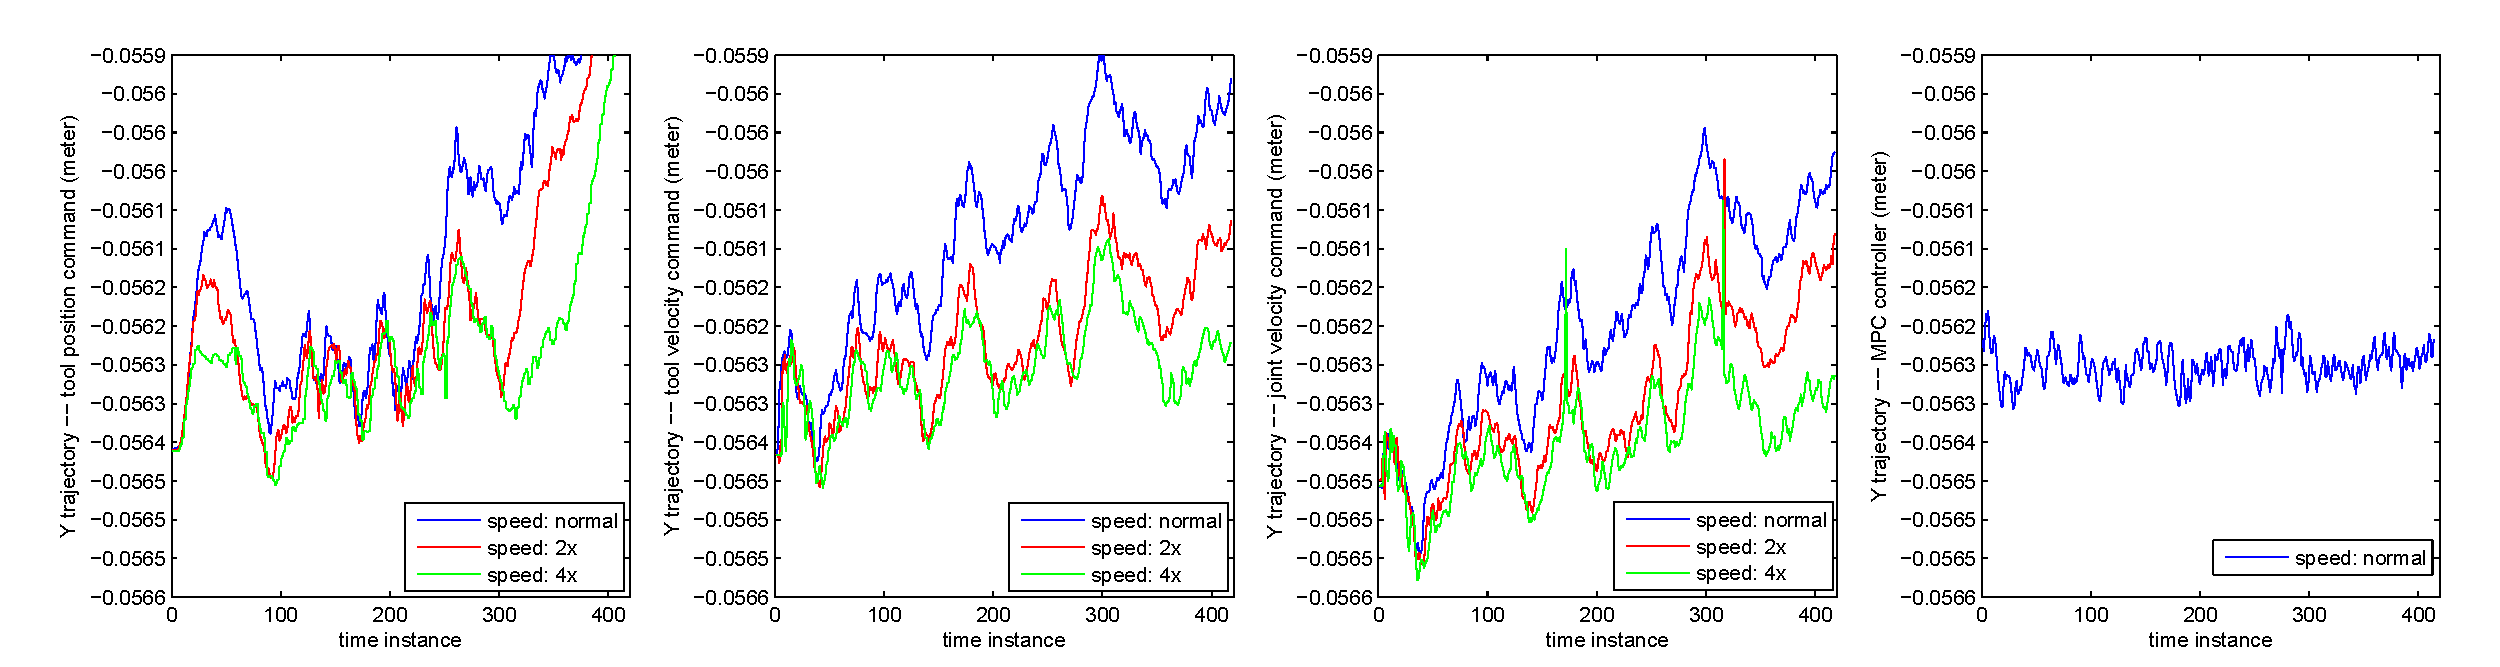
\includegraphics[width=0.9\linewidth]{images/trajectory_data_Y.pdf}
						\caption{\fontsize{8}{4}\selectfont Y trajectories of the robot with different controllers}
						\label{fig:trajectory_data_Y}
					\end{figure}
					\begin{figure}
						\centering
						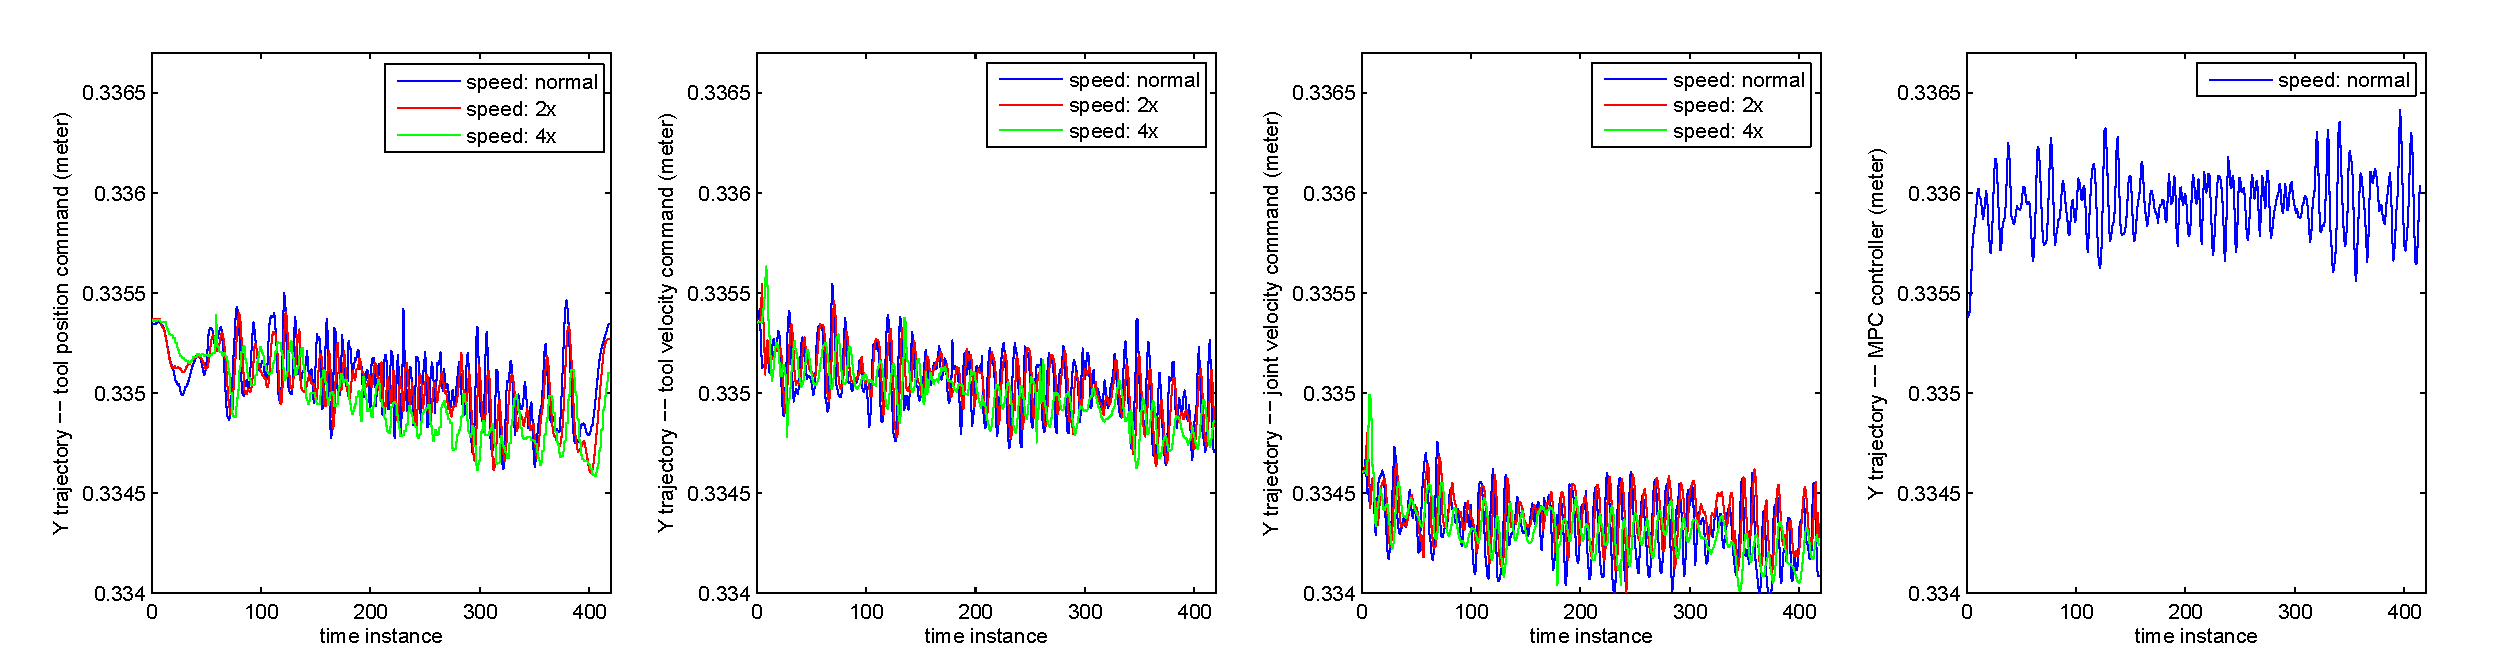
\includegraphics[width=0.9\linewidth]{images/trajectory_data_Z.pdf}
						\caption{\fontsize{8}{4}\selectfont Z trajectories of the robot with different controllers}
						\label{fig:trajectory_data_Z}
					\end{figure}
				\end{itemize}
			\end{frame}		
				
			\begin{frame}\frametitle{Hypotheses}
				\vspace{2mm}
				\begin{itemize}
					\fontsize{8}{4}\selectfont
					\item \textit{"Current controller (MPC) relies heavily on the identified model which is not perfect. Therefore, the model-mismatch induced by the unknown dynamics is responsible for the non-optimal performance of the MPC controller" }
					\vspace{3mm}
					\item \textit{"The best nominal controller yet is not PID, LQR, or else. It is the internal controller of the robot itself"}
					
				\end{itemize}
			\end{frame}
									
			\section{RL for Tracking: A Survey}
			\begin{frame}\frametitle{RL for Optimal Tracking Control}
				
				Assume a SISO LQT problem: \\
				\begin{equation} 
				\begin{split}
				x_{k+1} &= Ax_k + Bu_k \\
				y_k &= Cx_k \\
				\end{split}
				\end{equation}		
				with reference signal $ r_k $. \\
				\vspace{1mm}
				\begin{definition}
					The cost function:
					\begin{equation}
					J = V(x_k, r_k) := \frac{1}{2} \sum_{i=k}^{\infty} \Big(Cx_i-r_i\Big)^TQ\Big(Cx_i-r_i\Big) + {u_i}^TRu_i
					\end{equation}
				\end{definition}
			\end{frame}
			
			\begin{frame}\frametitle{RL for Optimal Tracking Control (2)}
				\fontsize{8}{4}\selectfont
				The solution to LQT is a combination of feedback and feedforward term: 
				\begin{equation} 
				u_{k} = -Kx_k + K_vv_{k+1} 
				\end{equation}		
				where
				\begin{equation}
				v_k = (A-BK)^Tv_{k+1} + C^TQr_k
				\end{equation}\vspace{1mm}
				
				The control gains are:
				\begin{equation}
				\begin{split}
				K &= (B^TSB + R)^{-1}B^TSA \\
				K_v &= (B^TSB + R)^{-1}B^T
				\end{split}
				\end{equation}
				with $S$ is the solution of ARE:
				\begin{equation}
				S = A^TSA - A^TSB(B^TSB+R)^{-1}B^TSA + C^TQC
				\end{equation}
				\fontsize{9}{4}\selectfont	
				\textbf{Drawback:} Have to solve a non-causal difference equation 
			\end{frame}
			
			\begin{frame}\frametitle{RL for Optimal Tracking Control (3)}
				\vspace{3mm}
				\fontsize{8}{4}\selectfont
				Important assumption:
				\begin{equation}
				r_{k+1} = Fr_k
				\end{equation}
				Construct an augmented state:
				\begin{equation}
				\begin{split}
				\left[ \begin{array}{c}
				x_{k+1} \\ 
				r_{k+1}
				\end{array} \right] &= \left[\begin{array}{cc}
				A & \text{0} \\ 
				\text{0} & F
				\end{array}  \right] \left[ \begin{array}{c}
				x_k \\ 
				r_k
				\end{array} \right] + \left[ \begin{array}{c}
				B \\ 
				\text{0}
				\end{array} \right] u_k \\
				X_{k+1} &= TX_k + B_1u_k
				\end{split}
				\end{equation}
				\begin{definition}
					\fontsize{8}{4}\selectfont
					Define a lyapunov function:
					\begin{equation}
					V(x_k, r_k) = V(X_k) = \frac{1}{2}{X_k}^TPX_k
					\end{equation}
				\end{definition}
				\vspace{3mm}
				\fontsize{8}{4}\selectfont
				Combining the infinite cost with lyapunov function yields a Bellman equation for augmented LQT: 
				\begin{equation}
				{X_k}^TPX_k =  {X_k}^TQ_1X_k + {u_k}^TRu_k + {X_{k+1}}^TPX_{k+1}
				\end{equation}
			\end{frame}
			
			\begin{frame}\frametitle{RL for Optimal Tracking Control (4)}
				\fontsize{8}{4}\selectfont
				Taking the time derivative of LQT Bellman, we obtain the LQT ARE
				\begin{equation}
				Q_1 - P + T^TPT - T^TPB_1(R+{B_1}^TPB_1)^{-1}{B_1}^TPT = 0
				\end{equation}
				
				The optimal policy is given by:
				\begin{equation}
				u_k = -K_1X_k
				\end{equation}
				with
				\begin{equation}
				K_1 = (R+{B_1}^TPB_1)^{-1}{B_1}^TPT
				\end{equation}	
				and 
				\begin{equation}
				Q_1 = \left[ \begin{array}{cc}
				C^TQC & -C^TQ \\ 
				-QC & Q
				\end{array} \right] 
				\end{equation}
				
			\end{frame}
			%\subsection{Section 1 - Subsection 3}
			
			\begin{frame}\frametitle{RL for Optimal Tracking Control (5)}
			\vspace{3mm}
			\fontsize{8}{4}\selectfont 
			From the LQT, obtain lyapunov equation
			\begin{equation}
				P =  Q_1 + {K_1}^TRK_1 + (T - B_1K_1)^TP(T - B_1K_1)
			\label{eq:lyap_equation}
			\end{equation}		
			Solve for $ P $ which satisfies \eqref{eq:lyap_equation}
			
			\begin{algorithm}[H]
			\begin{algorithmic}[1] 	
				\fontsize{8}{4}\selectfont			
				\STATE \textbf{Initialization:} Select an admissible (stable) gain ${K_1}^0$
				\REPEAT
					\STATE 	\textbf{Policy evaluation:} 
					\STATE 	$P^{j+1} = Q_1 + ({K_1}^j)^TRK_1^j + (T-B_1{K_1}^j)^TP^{j+1}(T-B_1{K_1}^j)$
					\STATE 	
					\STATE 	\textbf{Policy improvement:} 
					\STATE 	$ {K_1}^{j+1} = (R+{B_1}^TP^{j+1}B_1)^{-1} {B_1}^TP^{j+1}T $	
				\UNTIL{$ P $ converges}
				\caption{Offline Policy Iteration}
			\end{algorithmic}
			\end{algorithm}
			
%			\begin{algorithm}[H]
%			\begin{algorithmic}[1] 	
%				\fontsize{8}{4}\selectfont			
%				\STATE \textbf{Initialization:} Select an admissible (stable) gain $K^0_1$
%				\REPEAT
%					\STATE 	\textbf{Policy evaluation:} 
%					\STATE 	$X(k)^TP^{j+1}X(k) = X(k)^T\left( Q_1 + (K_1^j)^TRK_1^j\right) X(k) + X(k+1)^TP^{j+1}X(k+1)$
%					\STATE 	
%					\STATE 	\textbf{Policy improvement:} 
%					\STATE 	$ K_1^{j+1} = (R+B_1^TP^{j+1}B_1)^{-1} B_1^TP^{j+1}T $	
%				\UNTIL {$ P $ converges}
%				\caption{Online Policy Iteration}
%			\end{algorithmic}
%			\end{algorithm}			
			\end{frame}
			
			\begin{frame}\frametitle{RL for OTC with unknown system dynamics}
				\vspace{3mm}
				\fontsize{8}{4}\selectfont 
				\begin{itemize}
					\item Use a temporal difference (TD) RL technique 
 				\end{itemize}
				\begin{definition}
				Q-function: 
				\begin{equation}
				Q(X(k), u(k)) = \frac{1}{2}X(k)^TPX(k) 
				\label{eq:lyap}
				\end{equation}			
				\end{definition}
				
				Combining \eqref{eq:lyap} with Bellman yields:
				\begin{equation}
				\begin{split}
				Q(X(k), u(k)) &= \frac{1}{2}X(k)^TQ_1X(k) + \frac{1}{2}u(k)^TRu(k) + \frac{1}{2}\gamma X^T(k+1)PX(k+1) \\
				&= \frac{1}{2}X(k)^TQ_1X(k) + \frac{1}{2}u(k)^TRu(k) + \frac{1}{2}\gamma (TX(k) + B_1u(k))^TP(TX(k) + B_1u(k)) \\
				&= \frac{1}{2}\left[  \begin{array}{c}
				X(k) \\ 
				u(k)
				\end{array} \right] ^T \left[\begin{array}{cc}
				Q_1+\gamma T^TPT & \gamma T^TPB_1 \\ 
				\gamma B_1^TPT & R+\gamma B_1^TPB_1
				\end{array}  \right] 
				\left[  \begin{array}{c}
				X(k) \\ 
				u(k)
				\end{array} \right] 
				\end{split}
				\label{eq:bellman_Q}
				\end{equation}				
			\end{frame}			
			
			\begin{frame}\frametitle{RL for OTC with unknown system dynamics (2)}
				\vspace{3mm}
				\fontsize{8}{4}\selectfont 
				By defining:
				\begin{equation}
				H =  \left[\begin{array}{cc}
				Q_1+\gamma T^TPT & \gamma T^TPB_1 \\ 
				\gamma B_1^TPT & R+\gamma B_1^TPB_1
				\end{array}  \right] 
				=\left[ \begin{array}{cc}
				H_{XX} & H_{Xu} \\
				H_{uX} & H_{uu}
				\end{array} \right] 
				\end{equation}
				The optimal input is reached when $ \frac{\partial Q(X(k), u(k))}{\partial u(k)} = 0 $ which yields:
				\begin{equation}
				u(k) = -H_{uu}^{-1}H_{uX}X(k)
				\end{equation} 
				Fortunately, one can apply PI to solve for $ H $:
				\begin{algorithm}[H]
					\begin{algorithmic}[1]
						\fontsize{8}{4}\selectfont
						\STATE \textbf{Initialization:} Select an initial admissible (stable) control input $u = -K^0_1X_0$
						\REPEAT
						\STATE \textbf{Policy evaluation:} 
						\STATE $Z(k)^TH^{j+1}Z(k) = X(k)^TQ_1X(k) + (u(k)^j)^TRu(k)^j + Z(k+1)^THZ(k+1)$
						\STATE \textbf{Policy improvement:} 
						\STATE $ u^{j+1}(k) = -(H_{uu}^{-1})^{j+1} H_{uX}^{j+1}X(k) $ 
						\UNTIL{$ H $ converges}
						\caption{Model-free Policy Iteration}
					\end{algorithmic}			
				\end{algorithm}
			\end{frame}
			
			\begin{frame}\frametitle{RL for OTC: Summary}				
				\vspace{3mm}
				\textbf{Advantages:}
				\begin{itemize}
					\item Mathematically rigorous
					\item Proven to converge 
				\end{itemize}
				\vspace{3mm}
				\textbf{Disadvantages:}
				\begin{itemize}
					\item non-linear RL-based OTC does not exist 
					\item Needs a persistently exciting input, could be dangerous for the robot				
				\end{itemize}
			\end{frame}				
							
			\begin{frame}\frametitle{Dynamic Tuning via RL}
				\vspace{3mm}
				\fontsize{9}{4}\selectfont 
				\begin{itemize}
					\item A feedback control e.g. PID performs well at a certain region
					\item For different regions, the controller needs to be retuned
					\item Solution: gain scheduling
					\item The general diagram:
				\pause
				\begin{center}
					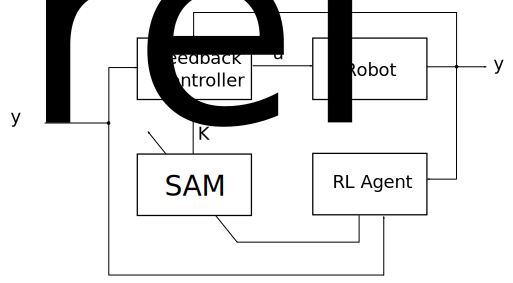
\includegraphics[width=0.70\linewidth]{images/dynatuning_block}
%					\caption{figure courtesy of }
					\hspace{5mm}
				\end{center}
				
				\item Various types of RL algorithm can be used: actor-critic, SARSA, etc
				\end{itemize}
			\end{frame}
			
			\begin{frame}\frametitle{Dynamic Tuning via RL (2): SARSA}
				\vspace{3mm}
				\fontsize{8}{4}\selectfont 
				\begin{itemize}
					\item Stands for state-action-reward-state-action
					\item Policy $\pi$ as gain modifier, not controller
				\end{itemize}
				\begin{center}
					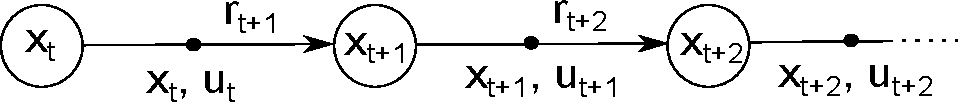
\includegraphics[width=0.50\linewidth]{images/sarsa}
					%					\caption{figure courtesy of }
				\end{center}
				\begin{algorithm}[H]
					\begin{algorithmic}[1] 	
						\fontsize{7}{4}\selectfont
						\STATE \textbf{Initialization:} Initialize $ Q(x,u) $ arbitrarily
						\REPEAT %( for each episode:)
							\STATE Initialize $ x $ 
							\STATE update $\pi$ based on $ Q $
							\STATE Choose $ K $ at $ x $ using $ \pi $  
							\REPEAT % ( for each step of episode:)
								\STATE Modify feedback controller using gain $ K $
								\STATE Take action $ u $ from the controller, observe $ r $, $ x' $ 
								\STATE update $ \pi $ based on $Q$
								\STATE Choose $ K' $ from $ x' $ using $ \pi $ 
								\STATE $ Q(x,K) \leftarrow Q(x,K) + \alpha[r+\gamma Q(x',K')-Q(x,K)] $	
								\STATE $ x \leftarrow  x' $
								\STATE $ K \leftarrow  K' $
							\UNTIL{$ x $ is terminal}
						\UNTIL{episodes run out}							
					\caption{SARSA algorithm}
					\end{algorithmic}						
				\end{algorithm}
			\end{frame}
			
			\begin{frame}\frametitle{Dynamic Tuning via RL (3): Actor-critic}
				\vspace{3mm}
				\fontsize{8}{4}\selectfont 
				\begin{itemize}
					\item An alternative to SARSA
					\item Actor and critic can be parameterized with a basis function e.g. RBF neural network
				\end{itemize}
				\begin{center}
					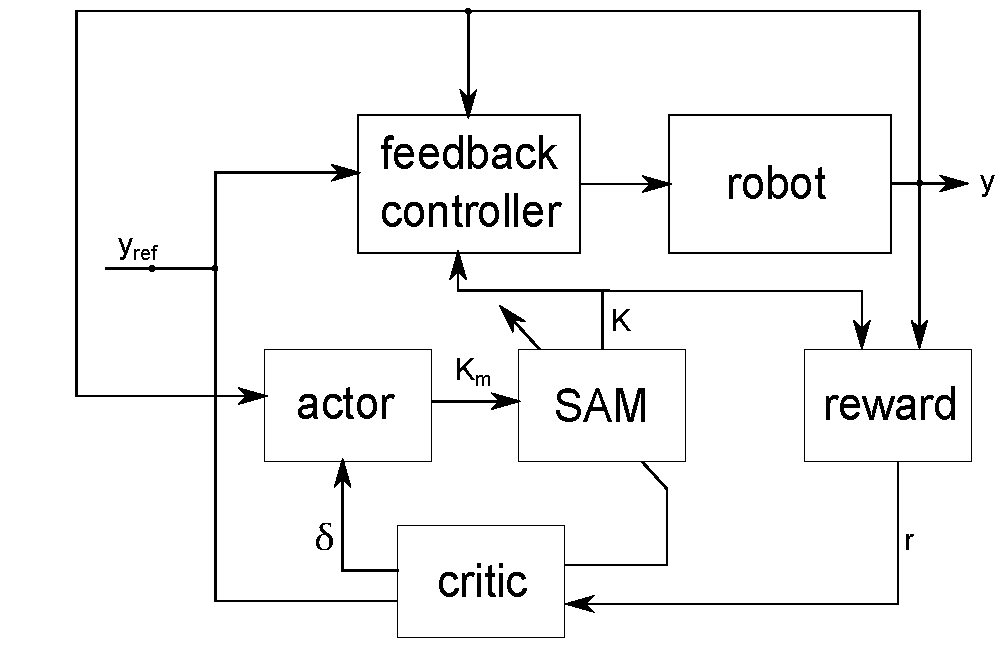
\includegraphics[width=0.70\linewidth]{images/actorcritic_dynamictuning}
					%					\caption{figure courtesy of }
				\end{center}
			\end{frame}			
			
			\begin{frame}\frametitle{Dynamic Tuning via RL (4): Summary}				
				\vspace{3mm}
				\textbf{Advantages:}
				\begin{itemize}
					\item Intuitive and easier to implement
				\end{itemize}
				\vspace{3mm}
				\textbf{Disadvantages:}
				\begin{itemize}
					\item so far only applies to feedback controller
					\item feedback controller "waits" until error occurs, hence it is always late
					\item  will not perform better due to this reason					
				\end{itemize}
			\end{frame}	
						
			\begin{frame}\frametitle{Nonlinear Compensator using RL}
				\vspace{3mm}
				\fontsize{8}{4}\selectfont 
				\begin{itemize}
					\item A relatively new approach
					\item Acts as an additive input
					\item An actor critic RL is proposed
					
					\begin{center}
						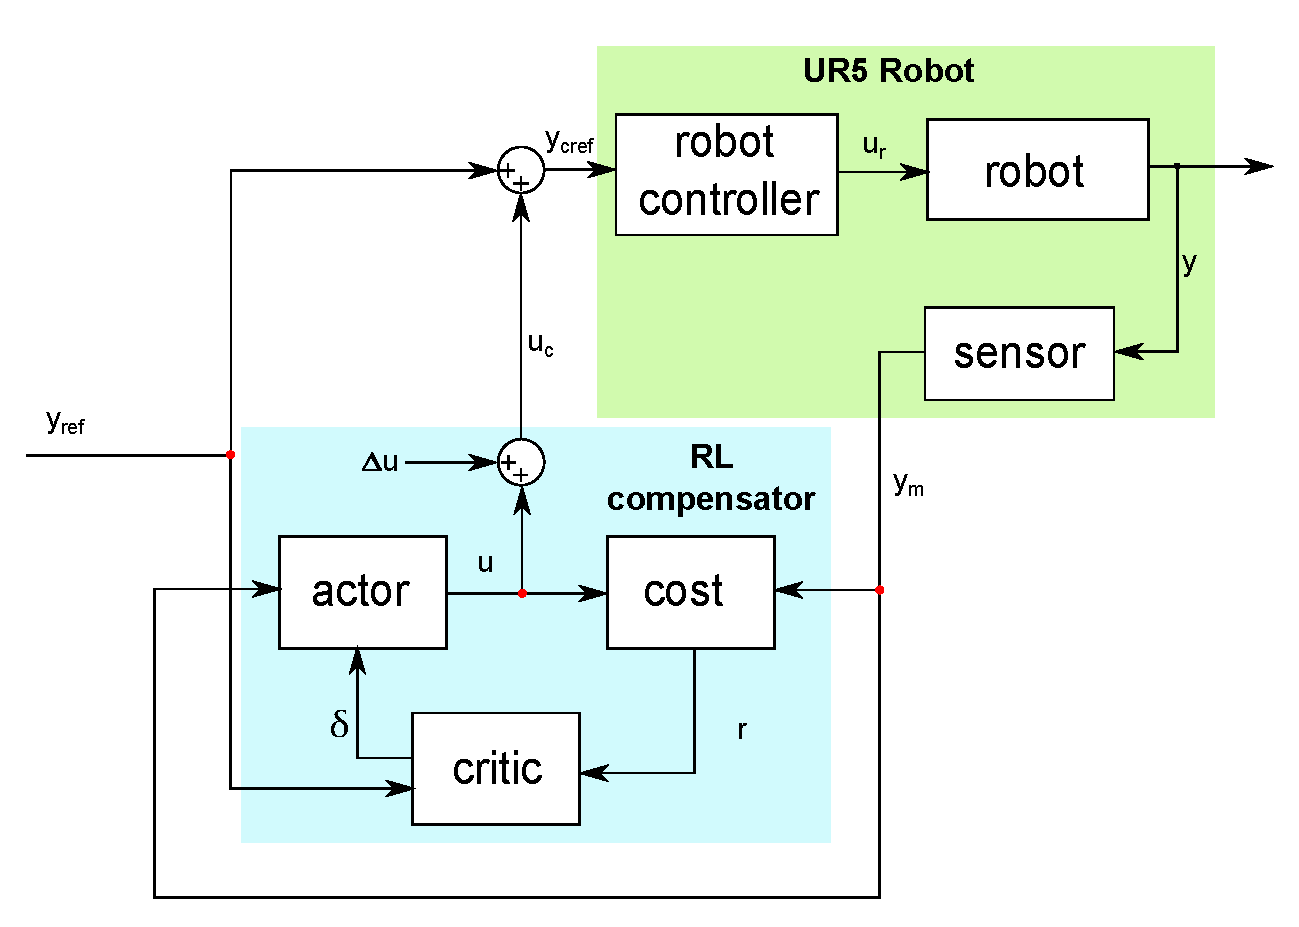
\includegraphics[width=0.80\linewidth]{images/nonlin_compensator}
						%					\caption{figure courtesy of }
					\end{center}
					\item Comparison with ILC is interesting
				\end{itemize}
				
			\end{frame}		
			
			\begin{frame}\frametitle{Nonlinear Compensator using RL (2)}
				\vspace{3mm}
				\fontsize{8}{4}\selectfont 
				\begin{itemize}
					\item cost function is defined to be similar to LQT
					\begin{equation}
					r_{k+1} = \rho(y_k, y^d_k, u_k) = (y^d_k - y_k)^TQ(y^d_k - y_k) + u_k^TRu_k
					\end{equation}
					\item Critic $V(x_k,\theta_k)$ and actor $\pi(x_k,\vartheta_{k-1})$ are parameterized by function approximators e.g. LLR, neural network, etc and  respectively.
				\end{itemize}
				\vspace{4mm}
				\textbf{Advantages:}
				\begin{itemize}
					\item a relatively new approach, hence interesting for research
					\item the compensator does not depend directly on the nominal control, hence adding a degree of freedom in control design 
				\end{itemize}
				\vspace{2mm}
				\textbf{Disadvantage:}
				\begin{itemize}
					\item Not mathematically as rigorous as RL-based optimal control 
				\end{itemize}
			\end{frame}											
			
			\section{Research Plan \& Conclusion}			
			\begin{frame}\frametitle{Research Plan}
				\begin{center}
					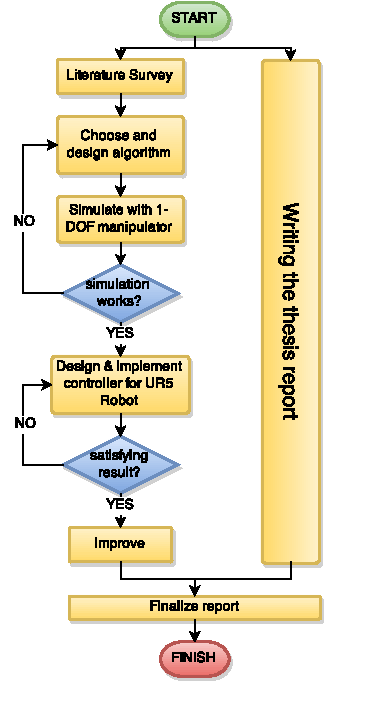
\includegraphics[width=0.35\linewidth]{images/research_plan}
				\end{center}
			\end{frame}

			\begin{frame}\frametitle{Conclusion}			
			\begin{itemize}
				\item The RL-based additive compensator is chosen as the most promising solution
				\item Simulation on 1-DoF arm will be performed before starting implementation on UR5 robot
				\item Possible comparison with ILC
			\end{itemize}
			\end{frame}		
			\begin{frame}\frametitle{End of presentation}			
					\centering
					Thank you for the attention \\
					\vspace{3mm}
					\fontsize{15}{4}\selectfont\textbf{ Question?}
			\end{frame}					
		\end{document}
		